\documentclass{beamer}

\usepackage[utf8]{inputenc}

\usepackage{tikz}
\usetikzlibrary{shapes,arrows}
\usetheme{AnnArbor}

\usepackage{graphicx}
\graphicspath{ {Figures/} }

%Information to be included in the title page:
\title{A decision support system for forecasting and optimal procurement}
\author{Neven Miculinić}
\date{July 2016}

\begin{document}

\frame{\titlepage}

% Present problem
% Present related work --> news vendor probelm
% Present related work --> news vendor dynamic lot sizing model
% Present solution to deterministic -> Naive approach
% Present solution to deterministic -> Transportation problem
% Present solution to deterministic -> Min cost max flow
% Present problem extensions
% Briefly talk about Time series analysis
% Briefly mentioned

\begin{frame}
\frametitle{Introduction}
\begin{itemize}
\item Decision maker has a factory which produces certain product with variable demand.
\item To produce the product it uses raw materials from supplier with variable cost.
\item There are cost penalties for storing raw material and for delaying demand satisfaction
\end{itemize}

% If there's extra raw materials it's stored and cost is payed per unit per day.

% If demand isn't satisfied backlogging cost is payed per unit per day until it's satisfied.

% His goal is minimizing total cost by deciding how much raw materials to purchase each time step.

\end{frame}


\begin{frame}
    \frametitle{Newsvendor problem}
    \begin{itemize}
        \item Inspired by newsvedor dilema.
        \item Product is perishable
    \end{itemize}

    \begin{block}{Formal definition}

        \begin{align*}
            D && \text{Random variable of product demand} \\
            s && \text{supply cost per unit} \\
            p && \text{selling price per unit} \\
        \end{align*}

        Variable is amount of perishable product to buy $x$.\\
        objective function:
        \begin{equation*}
            f = p\min(x, D) - sx
        \end{equation*}

    \end{block}
\end{frame}

\begin{frame}
    \frametitle{Dynamic lot sizing model}
    \begin{itemize}
        \item Similar to problem described in introduction
        \item Unlike original there's setup cost
    \end{itemize}

    \begin{block}{Formal definition}
        \begin{align*}
          d_t && \text{Demand at time period $t$} \\
          h_t && \text{Holding cost at time period $t$} \\
          K_t && \text{Setup cost at time period $t$} \\
          x^{(h)}_0 && \text{Initial inventory} \\
        \end{align*}

        and decision variable $\mathbf{x}$:
        \begin{align*}
                  x_t && \text{Quantity purchased at time period $t$}\\
        \end{align*}
    \end{block}
\end{frame}

\begin{frame}
    \frametitle{Dynamic lot sizing model}
    \begin{block}{}
        plus auxiliary variable $y_t$:
        \begin{equation*}
            y_t = \begin{cases}
                1 & x_t > 0\\
                0 & x_t = 0 \\
            \end{cases}
        \end{equation*}

        For simplicity we define inventory at time period $t$ as:

        \begin{align*}
          I_t &= x^{(h)}_0 + \sum_{t=0}^k{x_t} - \sum_{t=0}^k{d_t}\\
        \end{align*}

    \end{block}
\end{frame}

\begin{frame}
    \frametitle{Dynamic lot sizing model}
    \begin{block}{}
        And we want to choose optimal $x_t$, under following constraints:

        \begin{align*}
          x_t &\ge 0 \; \forall t\\
          I_t &\ge 0 \; \forall t\\
        \end{align*}

        And we want to minimize following objective function:
        \begin{equation*}
          f = \sum_t{h_t I_t + y_t K_t}
        \end{equation*}
    \end{block}
\end{frame}

\begin{frame}
    \frametitle{Formal problem definition}
    \begin{align*}
        \mathbf{s} &= \begin{bmatrix}
            s_1, s_2, \dotsc, s_n
        \end{bmatrix}^\intercal && \text{Supply cost vector} \\
        \mathbf{x} &= \begin{bmatrix}
            x_1, x_2, \dotsc, x_n
        \end{bmatrix}^\intercal && \text{Procurement quantity vector} \\
        \mathbf{x^{(\max)}}  & && \text{Procurement quantity limits vector} \\
        \mathbf{x}^{(b)}  & && \text{Backlogging quantity vector} \\
        \mathbf{x}^{(h)}  & && \text{Holding quantity vector} \\
        \mathbf{d} &= \begin{bmatrix}
            d_1, d_2, \dotsc, d_n
        \end{bmatrix}^\intercal && \text{Demand random vector} \\
        b & && \text{backlogging cost} \\
        h & && \text{holding cost} \\
        n & && \text{number of time moments}
    \end{align*}
\end{frame}

\begin{frame}
    \frametitle{Constraints}
    \begin{align*}
        x_t &\le x^{(\max)}_t & \forall t\\
        x_t &\ge 0 & \forall t\\
        x^{(b)}_t &\ge 0 & \forall t\\
        x^{(h)}_t &\ge 0 & \forall t\\
        x_t + x^{(h)}_{t - 1} + x^{(b)}_{t} &= d_t + x^{(h)}_t + h^{(b)}_{t - 1} & \forall t \\
        x^{(h)}_0 + x^{(b)}_n + \sum_{t=1}^n{x_i} &= \sum_{t=1}^n{d_i} + x^{(b)}_0 + x^{(h)}_n &\\
    \end{align*}
\end{frame}

\begin{frame}
    \frametitle{Objective function}
    \begin{itemize}
        \item \[c(t) = s_t x_t + b x^{(b)}_t + h x^{(h)}_t\]
        \item \[f =  \sum_t{c(t)} = \sum_t{ s_t x_t + b x^{(b)}_t + h x^{(h)}_t}\]
    \end{itemize}
\end{frame}

\begin{frame}
    \frametitle{Solution}
    \begin{itemize}
        \item Linear programming/Mixed integer programming
        \item Transportation problem
        \item \alert{Min cost max flow}
    \end{itemize}
\end{frame}

\begin{frame}[shrink=0.5]
    \frametitle{Min Cost max flow solution}
    \begin{figure}[h]
      \centering
      
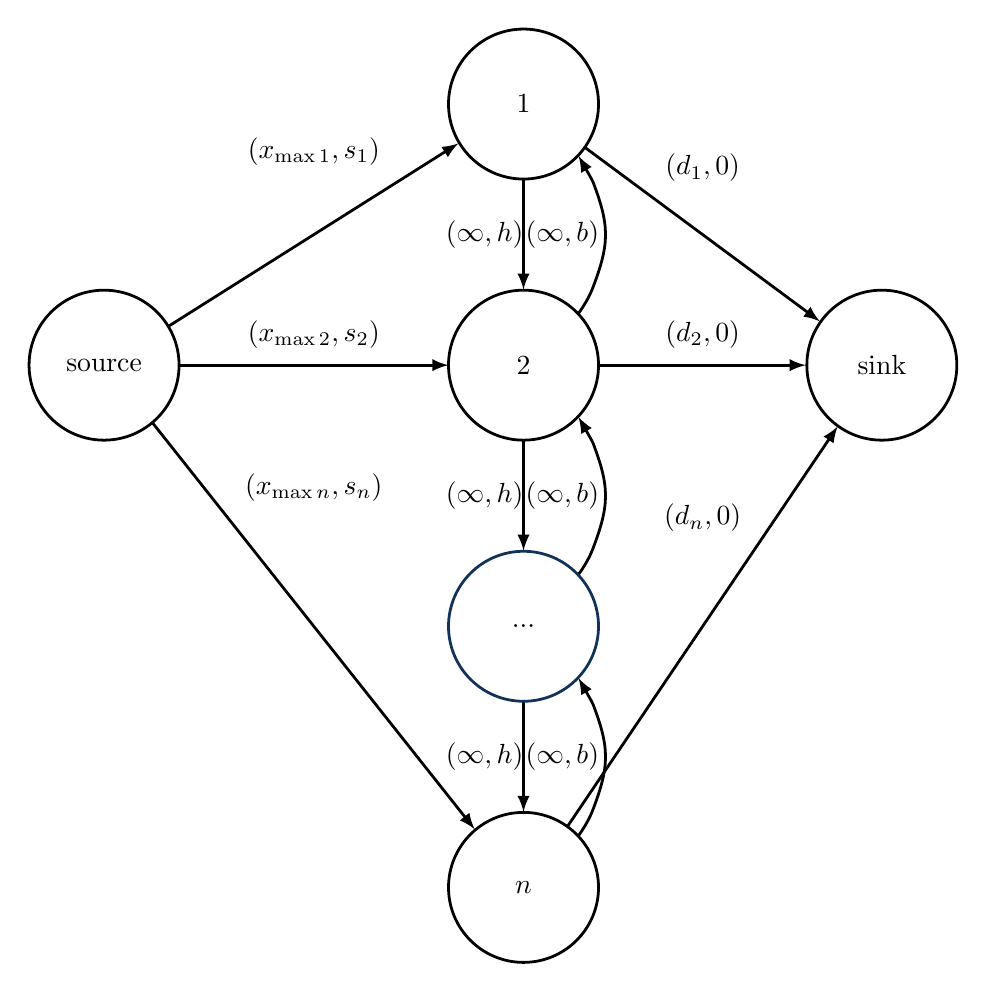
\begin{tikzpicture}[>=latex,line join=bevel,]
  \pgfsetlinewidth{1bp}
%%
\begin{scope}
  \pgfsetstrokecolor{black}
  \definecolor{strokecol}{rgb}{1.0,1.0,1.0};
  \pgfsetstrokecolor{strokecol}
  \definecolor{fillcol}{rgb}{1.0,1.0,1.0};
  \pgfsetfillcolor{fillcol}
  \filldraw (0.0bp,0.0bp) -- (0.0bp,336.0bp) -- (334.0bp,336.0bp) -- (334.0bp,0.0bp) -- cycle;
\end{scope}
\begin{scope}
  \pgfsetstrokecolor{black}
  \definecolor{strokecol}{rgb}{1.0,1.0,1.0};
  \pgfsetstrokecolor{strokecol}
  \definecolor{fillcol}{rgb}{1.0,1.0,1.0};
  \pgfsetfillcolor{fillcol}
  \filldraw (0.0bp,0.0bp) -- (0.0bp,336.0bp) -- (334.0bp,336.0bp) -- (334.0bp,0.0bp) -- cycle;
\end{scope}
  \pgfsetcolor{black}
  % Edge: n -> m
  \draw [->] (197.79bp,45.647bp) .. controls (199.91bp,48.565bp) and (201.75bp,51.712bp)  .. (203.0bp,55.0bp) .. controls (209.02bp,70.78bp) and (209.02bp,77.22bp)  .. (203.0bp,93.0bp) .. controls (202.92bp,93.205bp) and (202.84bp,93.41bp)  .. (197.79bp,102.35bp);
  \definecolor{strokecol}{rgb}{0.0,0.0,0.0};
  \pgfsetstrokecolor{strokecol}
  \draw (192.0bp,74.0bp) node {$(\infty, b)$};
  \draw (203.79bp,51.647bp) node {$$};
  \draw (203.79bp,96.353bp) node {$$};
  % Edge: m -> n
  \draw [->] (178.0bp,93.872bp) .. controls (178.0bp,84.622bp) and (178.0bp,74.113bp)  .. (178.0bp,54.189bp);
  \draw (164.0bp,74.0bp) node {$(\infty, h)$};
  \draw (184.0bp,90.872bp) node {$$};
  \draw (184.0bp,54.189bp) node {$$};
  % Edge: source -> 2
  \draw [->] (54.295bp,215.0bp) .. controls (78.339bp,215.0bp) and (114.12bp,215.0bp)  .. (150.97bp,215.0bp);
  \draw (102.5bp,226.0bp) node {$(x_{\max 2}, s_2)$};
  \draw (60.295bp,209.0bp) node {$$};
  \draw (144.97bp,209.0bp) node {$$};
  % Edge: 2 -> 1
  \draw [->] (197.79bp,233.65bp) .. controls (199.91bp,236.57bp) and (201.75bp,239.71bp)  .. (203.0bp,243.0bp) .. controls (209.02bp,258.78bp) and (209.02bp,265.22bp)  .. (203.0bp,281.0bp) .. controls (202.92bp,281.21bp) and (202.84bp,281.41bp)  .. (197.79bp,290.35bp);
  \draw (192.0bp,262.0bp) node {$(\infty, b)$};
  \draw (203.79bp,239.65bp) node {$$};
  \draw (191.79bp,284.35bp) node {$$};
  % Edge: n -> sink
  \draw [->] (193.82bp,48.934bp) .. controls (216.41bp,82.381bp) and (259.56bp,146.25bp)  .. (291.08bp,192.92bp);
  \draw (242.5bp,160.0bp) node {$(d_n, 0)$};
  \draw (187.82bp,42.934bp) node {$$};
  \draw (285.08bp,186.92bp) node {$$};
  % Edge: m -> 2
  \draw [->] (197.79bp,139.65bp) .. controls (199.91bp,142.57bp) and (201.75bp,145.71bp)  .. (203.0bp,149.0bp) .. controls (209.02bp,164.78bp) and (209.02bp,171.22bp)  .. (203.0bp,187.0bp) .. controls (202.92bp,187.21bp) and (202.84bp,187.41bp)  .. (197.79bp,196.35bp);
  \draw (192.0bp,168.0bp) node {$(\infty, b)$};
  \draw (203.79bp,145.65bp) node {$$};
  \draw (203.79bp,190.35bp) node {$$};
  % Edge: 2 -> m
  \draw [->] (178.0bp,187.87bp) .. controls (178.0bp,178.62bp) and (178.0bp,168.11bp)  .. (178.0bp,148.19bp);
  \draw (164.0bp,168.0bp) node {$(\infty, h)$};
  \draw (184.0bp,184.87bp) node {$$};
  \draw (184.0bp,148.19bp) node {$$};
  % Edge: 1 -> sink
  \draw [->] (200.26bp,293.27bp) .. controls (221.14bp,277.81bp) and (253.17bp,254.1bp)  .. (284.67bp,230.78bp);
  \draw (242.5bp,286.0bp) node {$(d_1, 0)$};
  \draw (206.26bp,287.27bp) node {$$};
  \draw (278.67bp,224.78bp) node {$$};
  % Edge: 1 -> 2
  \draw [->] (178.0bp,281.87bp) .. controls (178.0bp,272.62bp) and (178.0bp,262.11bp)  .. (178.0bp,242.19bp);
  \draw (164.0bp,262.0bp) node {$(\infty, h)$};
  \draw (184.0bp,281.87bp) node {$$};
  \draw (184.0bp,245.19bp) node {$$};
  % Edge: source -> n
  \draw [->] (44.515bp,194.16bp) .. controls (71.142bp,160.57bp) and (123.63bp,94.338bp)  .. (160.41bp,47.931bp);
  \draw (102.5bp,171.0bp) node {$(x_{\max n}, s_n)$};
  \draw (50.515bp,188.16bp) node {$$};
  \draw (154.41bp,53.931bp) node {$$};
  % Edge: source -> 1
  \draw [->] (50.307bp,229.07bp) .. controls (75.653bp,245.06bp) and (117.2bp,271.27bp)  .. (154.54bp,294.83bp);
  \draw (102.5bp,292.0bp) node {$(x_{\max 1}, s_1)$};
  \draw (56.307bp,223.07bp) node {$$};
  \draw (148.54bp,288.83bp) node {$$};
  % Edge: 2 -> sink
  \draw [->] (205.01bp,215.0bp) .. controls (223.63bp,215.0bp) and (248.96bp,215.0bp)  .. (279.59bp,215.0bp);
  \draw (242.5bp,226.0bp) node {$(d_2, 0)$};
  \draw (211.01bp,209.0bp) node {$$};
  \draw (273.59bp,209.0bp) node {$$};
  % Node: m
\begin{scope}
  \definecolor{strokecol}{rgb}{0.07,0.2,0.34};
  \pgfsetstrokecolor{strokecol}
  \draw (178.0bp,121.0bp) ellipse (27.0bp and 27.0bp);
  \definecolor{strokecol}{rgb}{0.0,0.0,0.0};
  \pgfsetstrokecolor{strokecol}
  \draw (178.0bp,121.0bp) node {$...$};
\end{scope}
  % Node: n
\begin{scope}
  \definecolor{strokecol}{rgb}{0.0,0.0,0.0};
  \pgfsetstrokecolor{strokecol}
  \draw (178.0bp,27.0bp) ellipse (27.0bp and 27.0bp);
  \draw (178.0bp,27.0bp) node {$n$};
\end{scope}
  % Node: 1
\begin{scope}
  \definecolor{strokecol}{rgb}{0.0,0.0,0.0};
  \pgfsetstrokecolor{strokecol}
  \draw (178.0bp,309.0bp) ellipse (27.0bp and 27.0bp);
  \draw (178.0bp,309.0bp) node {$1$};
\end{scope}
  % Node: source
\begin{scope}
  \definecolor{strokecol}{rgb}{0.0,0.0,0.0};
  \pgfsetstrokecolor{strokecol}
  \draw (27.0bp,215.0bp) ellipse (27.0bp and 27.0bp);
  \draw (27.0bp,215.0bp) node {source};
\end{scope}
  % Node: 2
\begin{scope}
  \definecolor{strokecol}{rgb}{0.0,0.0,0.0};
  \pgfsetstrokecolor{strokecol}
  \draw (178.0bp,215.0bp) ellipse (27.0bp and 27.0bp);
  \draw (178.0bp,215.0bp) node {$2$};
\end{scope}
  % Node: sink
\begin{scope}
  \definecolor{strokecol}{rgb}{0.0,0.0,0.0};
  \pgfsetstrokecolor{strokecol}
  \draw (307.0bp,215.0bp) ellipse (27.0bp and 27.0bp);
  \draw (307.0bp,215.0bp) node {sink};
\end{scope}
%
\end{tikzpicture}


      \caption{min cost max flow model. Arcs are labeled (capacity, cost)}
    \end{figure}
\end{frame}

\begin{frame}
    \frametitle{Problem variants}
    \begin{itemize}
        \item Starting storage capacity
        \item Ending storage requirement
        \item Allowing future backlogging
        \item Leap time ordering
        \item Multiple raw material suppliers
    \end{itemize}
\end{frame}

\begin{frame}
    \frametitle{Forecasting future data points}
    \begin{itemize}
        \item AR model
        \item MA model
        \item ARIMA model
        \item Model fitted using Akaike information criterion (AIC)
    \end{itemize}
\end{frame}

\begin{frame}
    \frametitle{Implementation and application}
    \begin{itemize}
        \item python API
        \item experimented on real dataset
    \end{itemize}
\end{frame}

\begin{frame}
    \frametitle{Americal coal prices}
    \begin{figure}[]
      \centering
      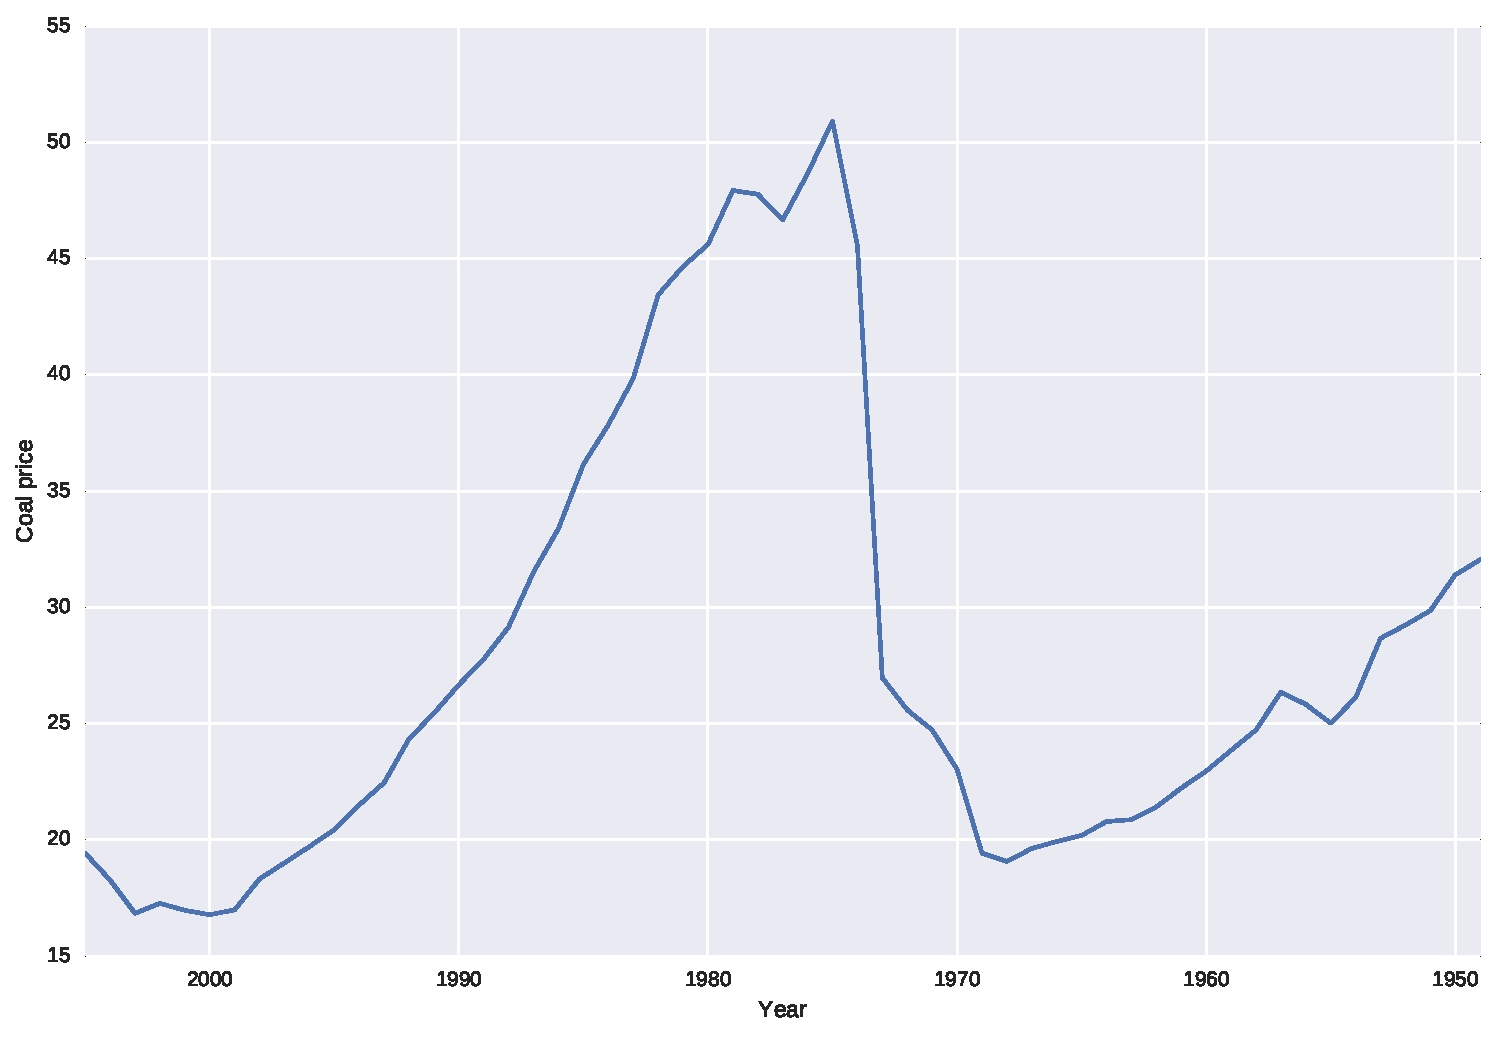
\includegraphics[width=0.8\linewidth]{supply}
          \caption{Yearly coal prices. Green are prediction with ARIMA(0,1,1) model}
    \end{figure}
\end{frame}


\begin{frame}
    \frametitle{US yearly electricity demand}
    \begin{figure}[]
      \centering
      \includegraphics[width=0.8\linewidth]{demand}
      \caption{Yearly electricity demand. Green are predictions with ARIMA(1,2,0) model}
    \end{figure}
\end{frame}
\end{document}
